\section{Our Approach} % (fold)
\label{sec:approach}

A typical phishing scenario starts with a fraudster sending an email to a potential victim. The end goal is to lure the user into clicking on a link to provide critical information regarding their banking details (e.g., online banking credentials, account number, identification details). Figure~\ref{fig:phishing-email} depicts a template of such an email.

\begin{figure}[hp!]
  \begin{center}
    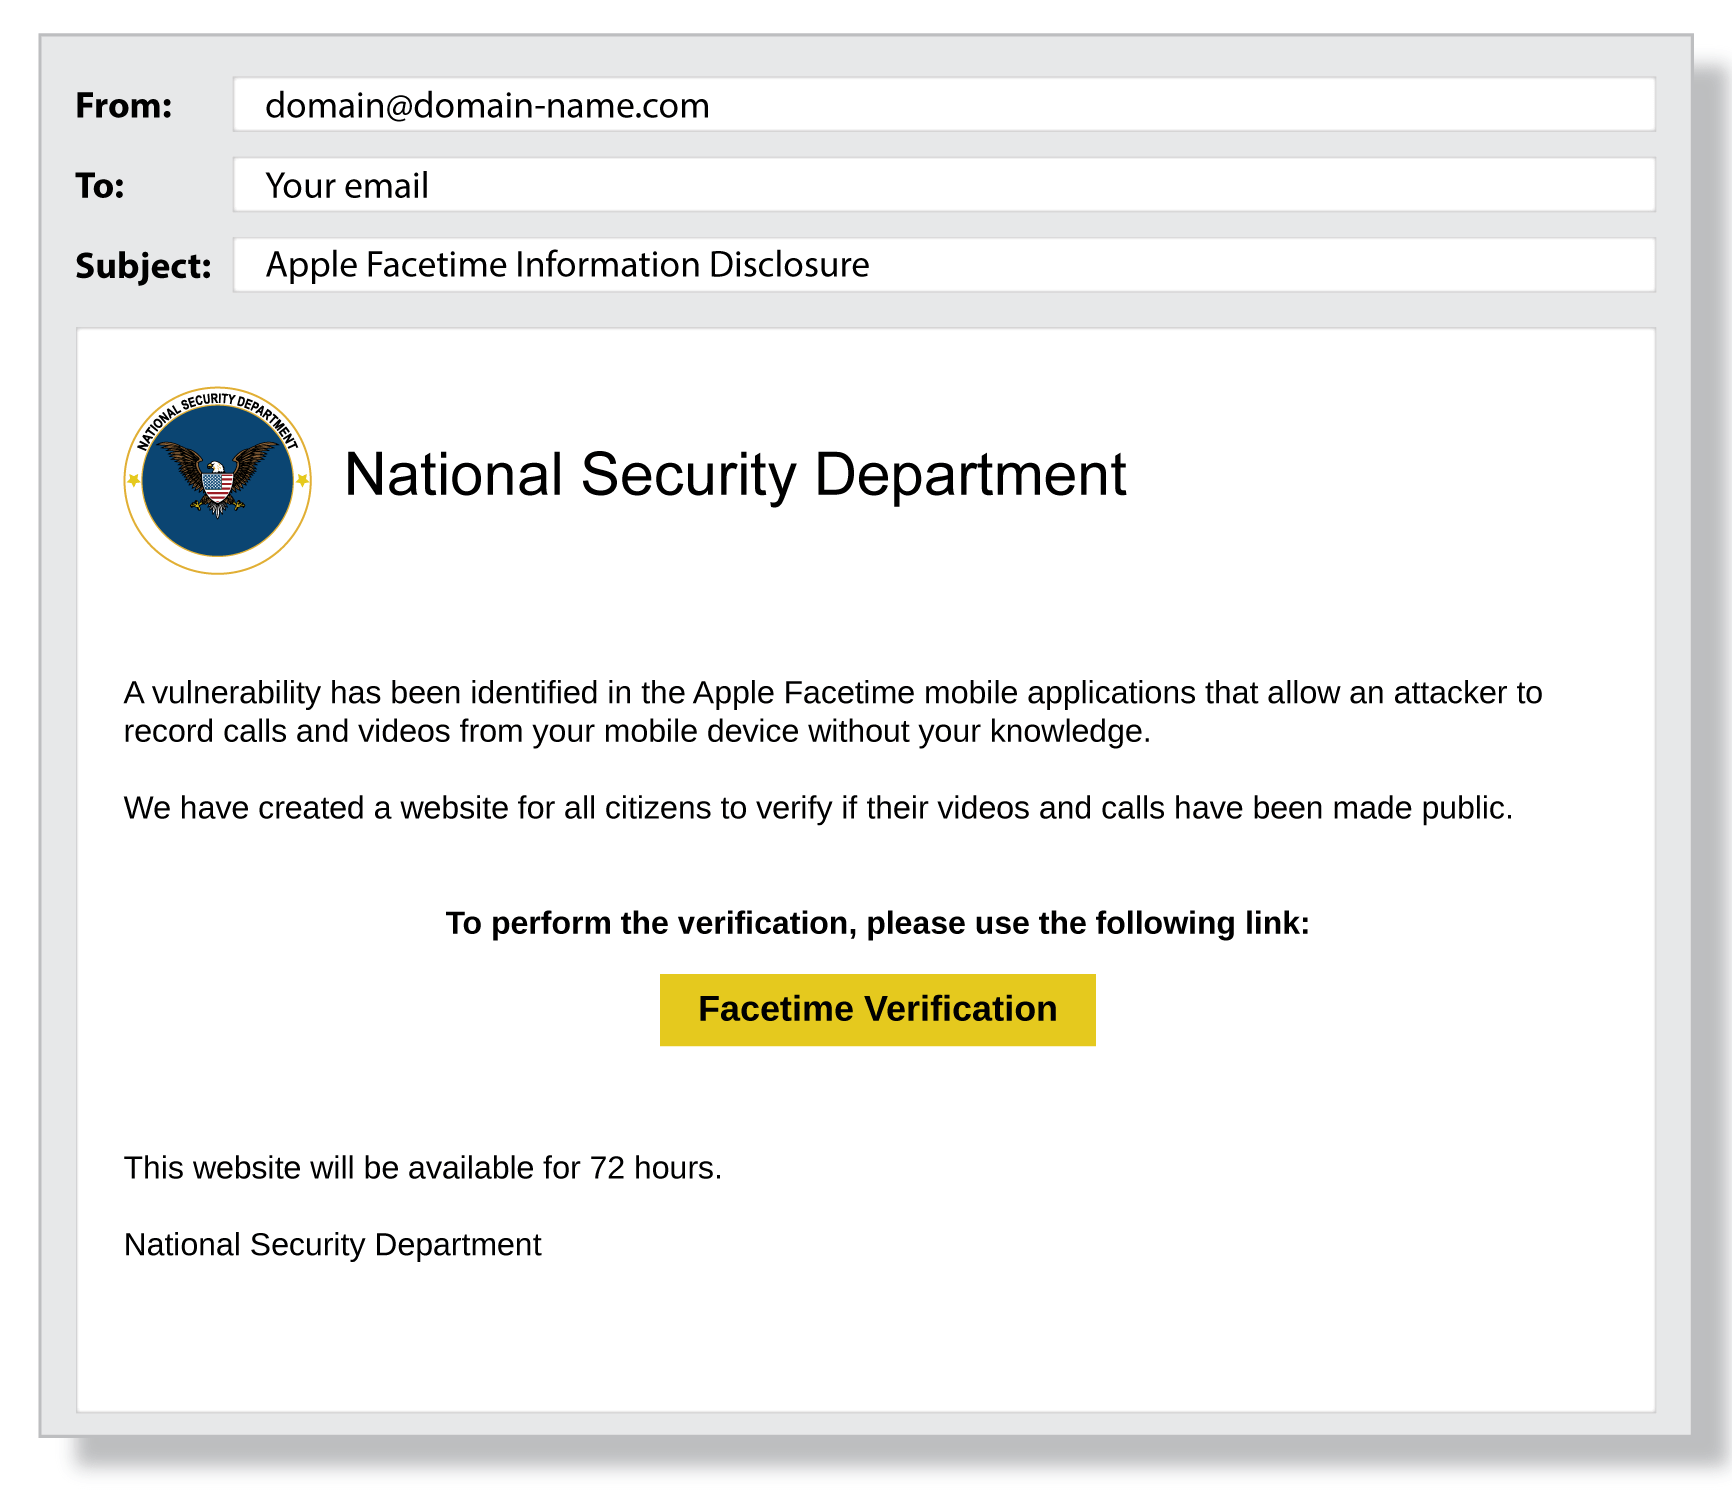
\includegraphics[width=0.85\textwidth]{phishing-email-eg}
  \end{center}
  \caption{Example of Phishing Email}\label{fig:phishing-email}
\end{figure}

We use a \gls{nlp}-based \emph{text analysis}\footnote{The text analysis algorithm is out of the scope of this paper.}  technique to understand the email and select the link(s). We strip each link of the protocol (e.g., HTTP, HTTPS) and query parameters and extract the \emph{domain name}. Next we analyse the domain name and look for similar phonetically-sounding domain names. Finally, we scrutinise the web forms corresponding to the identified domain names and assess their closeness. We discuss both techniques in this section.

\subsection{Link Analysis} % (fold)
\label{sub:approach-link-analysis}

We define a \emph{string} as a finite sequence of characters over an alphabet. We argue that two strings $\mathsf{s_1}$ and $\mathsf{s_2}$ are strings sharing some closeness in their representation. Definition~\ref{theo:phonetic-names} defines phonetic similarity in our context.  

\begin{definition}[Phonetically Similar Strings]
  \label{theo:phonetic-names}
  Given a string $\mathsf{S}$, a string $\mathsf{S^\prime}$ sounds phonetically similar to $\mathsf{S}$ if  $\mathsf{S^\prime}$ is a \emph{sub-string} of $\mathsf{S}$ starting from the same character, or $\mathsf{S^\prime}$ is a \emph{super-string} of $\mathsf{S}$.  
\end{definition}

For example, given the string {\texttt{standardbank}}, {\texttt{standardbank1}} is phonetically similar as a super-string; {\texttt{standarbank}} is also phonetically similar as a sub-string with an inexact match. We execute the the match operation (both exact and inexact) using  a \emph{trie}~\cite{leis-kemper-neumann:2013,morrison:1968,gusfield:1997,ukkonen:1995} data structure. A trie (or suffix tree) is a \emph{hierarchical} data structure used to efficiently represent a string and its suffixes.

We expand the English alphabet with digits (alphanumeric) and a specical character admitted in domain names. Let $\Sigma$ represent our new alphabet; $\Sigma = \{a, b, \ldots, z\}~\bigcup~\{0, 1, \ldots, 9\}~\bigcup~\{-\}$. We construct the suffix tree following Ukkonen's algorithm~\cite{ukkonen:1995}. The construction algorithm starts with a root node. For each character in the string, a new edge is added. These edges are combined (or compressed) to avoid longer paths. 


A match operation visits the trie from the root all the way to the leaves.  



\begin{definition}[Super Strings]
  \label{theo:super-strs}
  Given a string $\mathsf{Nm}$, a super-string of $\mathsf{Nm}$ is a string whose suffixes include $\mathsf{Nm}$.
\end{definition}





A sorted list of suffixes for the string {\texttt{standardbank}} is $\{\texttt{andardbank}, \texttt{ank}, \texttt{ardbank}, \texttt{bank}, \texttt{dardbank}, \texttt{dbank}, \texttt{k}, \texttt{ndardbank}, \texttt{nk}, \texttt{rdbank}, \texttt{tandardbank}\}$.


\SetKwInput{KwInput}{Input}
\SetKwInput{KwOutput}{Output}

\begin{algorithm}[pth]
    \DontPrintSemicolon
    \KwInput{$\mathsf{N}$ \atcp{Initial solution size}}
    \KwInput{$\mathsf{M}$ \atcp{Iteration count}}
    \KwInput{$\mathsf{Ope}$ \atcp{MAX or MIN}}
    \KwOutput{$\mathsf{C}$ \atcp{New clusters}}

    $\mathsf{I} \gets \mathit{generate\_initial\_solutions}(\mathsf{N})$\;

    $\mathrm{I} \gets \mathit{compute\_brightness}(\mathsf{I})$\;

    \For{$iter=1,\ldots ,\mathsf{M}$}{
      \For{$\imath = 1,\ldots ,\mathsf{N}$}{
        \For{$\jmath = 1, \ldots ,\mathsf{N}$}{
          \If{$\imath \neq \jmath$}{
            \If{$\mathsf{Ope} == MAX$}{
              \If{$\mathsf{I}(\imath).brightness < \mathsf{I}(\jmath).brightness$}{
                $\mathit{update\_position}(\imath, \jmath)$\;
              }
            }

            \If{$\mathsf{Ope} == MIN$}{
              \If{$\mathsf{I}(\imath).brightness > \mathsf{I}(\jmath).brightness$}{
                $\mathit{update\_position}(\imath, \jmath)$\;
              }
            }
          }
        }
      }
    }
    
    $\mathsf{C}\gets\mathit{extract\_clusters}(\mathsf{I})$\;

    $\KwRet~~\mathsf{C}$\;

    \SetKwProg{fn}{Function}{}{}
    \SetKwFunction{initatenegofunc}{$\mathit{initiate\_negotiation}$}{}
    \SetKwFunction{handlemsgfunc}{$\mathit{handle\_message}$}{}
    \;

\caption{Refuse Item Clustering}
\label{alg:fa-clustering}
\end{algorithm}


We construct the suffix tree of the domain name and extract all the suffixes related to it.

In addition... talk about the superstring part of the domain name

Could envision a map-reduce architecture for solving the overall queries to 


% subsection Link Analysis (end)

\subsection{Web Page Analysis} % (fold)
\label{sub:approach-web-page-analysis}

Here we discuss how we generate the graph and check similarity using a GNN

% subsection Web Page Analysis (end)

% section Our Approach (end)
